\begin{figure}[tbp]
\centering
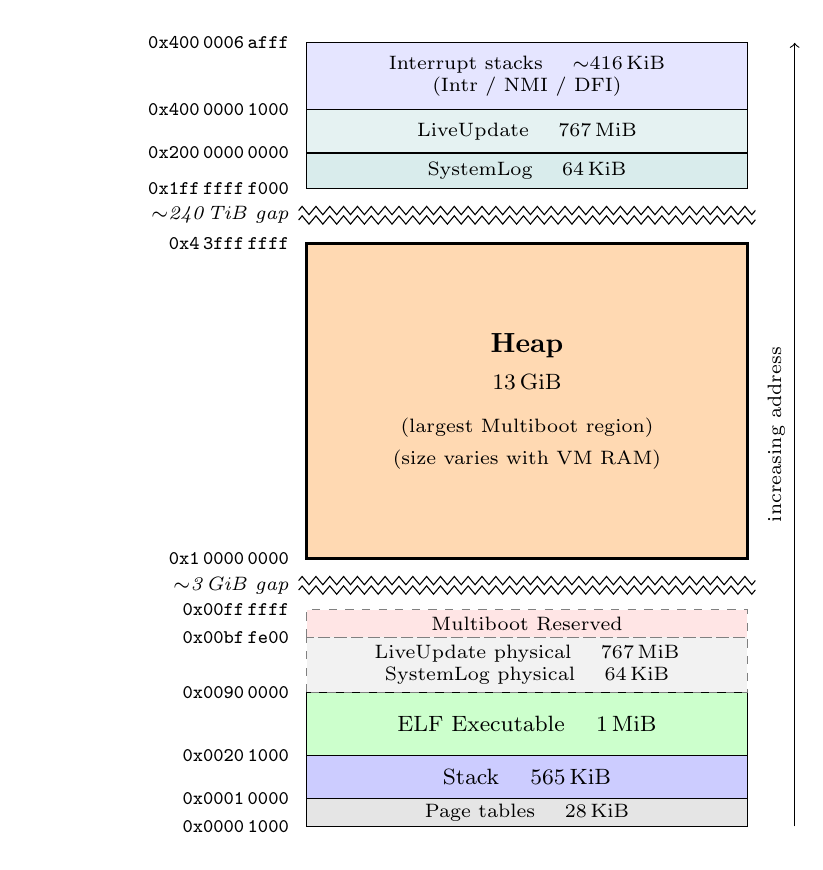
\begin{tikzpicture}[
  every node/.style={font=\footnotesize},
  addr/.style={anchor=east, font=\ttfamily\scriptsize,
               text width=3.2cm, align=right},
]

%% --- Zone 1: low addresses (0 -- ~1 GiB) ---

\draw[fill=gray!20]  (0,0.00) rectangle (5.6,0.35);
\node[font=\scriptsize] at (2.8,0.175) {Page tables \quad 28\,KiB};
\node[addr] at (-0.1,0.00) {0x0000\,1000};

\draw[fill=blue!20]  (0,0.35) rectangle (5.6,0.90);
\node at (2.8,0.625) {Stack \quad 565\,KiB};
\node[addr] at (-0.1,0.35) {0x0001\,0000};

\draw[fill=green!20] (0,0.90) rectangle (5.6,1.70);
\node at (2.8,1.30) {ELF Executable \quad 1\,MiB};
\node[addr] at (-0.1,0.90) {0x0020\,1000};

\draw[fill=gray!10, draw=gray, dashed] (0,1.70) rectangle (5.6,2.40);
\node[font=\scriptsize, align=center] at (2.8,2.05)
  {LiveUpdate physical \quad 767\,MiB\\SystemLog physical \quad 64\,KiB};
\node[addr] at (-0.1,1.70) {0x0090\,0000};

\draw[fill=red!10, draw=gray, dashed] (0,2.40) rectangle (5.6,2.75);
\node[font=\scriptsize] at (2.8,2.575) {Multiboot Reserved};
\node[addr] at (-0.1,2.40) {0x00bf\,fe00};
\node[addr] at (-0.1,2.75) {0x00ff\,ffff};

%% --- Axis break 1 ---
\foreach \yy in {3.00,3.12} {
  \draw[decorate,decoration={zigzag,amplitude=1.5pt,segment length=5pt}]
    (-0.1,\yy) -- (5.7,\yy);
}
\node[anchor=east, font=\scriptsize\itshape] at (-0.1,3.06) {$\sim$3\,GiB gap};

%% --- Zone 2: Heap ---
\draw[fill=orange!30, thick] (0,3.40) rectangle (5.6,7.40);
\node[align=center] at (2.8,5.40)
  {\normalsize\textbf{Heap}\\[4pt]
   13\,GiB\\[6pt]
   \scriptsize (largest Multiboot region)\\[2pt]
   \scriptsize (size varies with VM RAM)};
\node[addr] at (-0.1,3.40) {0x1\,0000\,0000};
\node[addr] at (-0.1,7.40) {0x4\,3fff\,ffff};

%% --- Axis break 2 ---
\foreach \yy in {7.70,7.82} {
  \draw[decorate,decoration={zigzag,amplitude=1.5pt,segment length=5pt}]
    (-0.1,\yy) -- (5.7,\yy);
}
\node[anchor=east, font=\scriptsize\itshape] at (-0.1,7.76) {$\sim$240\,TiB gap};

%% --- Zone 3: high addresses ---
\draw[fill=teal!15] (0,8.10) rectangle (5.6,8.55);
\node[font=\scriptsize] at (2.8,8.325) {SystemLog \quad 64\,KiB};
\node[addr] at (-0.1,8.10) {0x1ff\,ffff\,f000};

\draw[fill=teal!10]  (0,8.55) rectangle (5.6,9.10);
\node[font=\scriptsize] at (2.8,8.825) {LiveUpdate \quad 767\,MiB};
\node[addr] at (-0.1,8.55) {0x200\,0000\,0000};

\draw[fill=blue!10]  (0,9.10) rectangle (5.6,9.95);
\node[font=\scriptsize, align=center] at (2.8,9.525)
  {Interrupt stacks \quad $\sim$416\,KiB\\(Intr / NMI / DFI)};
\node[addr] at (-0.1,9.10)  {0x400\,0000\,1000};
\node[addr] at (-0.1,9.95) {0x400\,0006\,afff};

%% --- Increasing-address arrow ---
\draw[->] (6.2,0.00) -- (6.2,9.95)
  node[midway, rotate=90, anchor=south, font=\scriptsize] {increasing address};

\end{tikzpicture}
\caption{Virtual address space layout of an IncludeOS instance after boot (16\,GiB VM).
  Regions are not drawn to scale; axis breaks indicate large gaps in the address space.
  The heap occupies the largest contiguous region reported by the Multiboot memory map,
  starting just above the 4\,GiB boundary; its size depends on the amount of memory
  assigned to the virtual machine. Everything below it is set up by the
  bootloader and early boot code before any allocator exists.
  \Cref{sec:includeos-memory-model} walks through how each region gets
  there.}
\label{fig:address-space}
\end{figure}



%%  0x0000001000 - 0x0000007fff,  28.000_KiB (100.0 %) Page tables
%%  0x0000010000 - 0x000009d3ff, 565.000_KiB (100.0 %) Stack
%%  0x000009fc00 - 0x000009ffff,   1.000_KiB (100.0 %) UNALIGNED
%%  0x00000f0000 - 0x00000fffff,  64.000_KiB (100.0 %) Multiboot (Reserved)
%%  0x0000201000 - 0x0000315fff,   1.082_MiB (100.0 %) ELF Executable (Unikernel service)
%%  0x0001000000 - 0x0005feefff,  79.934_MiB (2.243 %) Heap
%%  0x00060ef000 - 0x00060fefff,  64.000_KiB (100.0 %) SystemLog physical
%%  0x00060ff000 - 0x0007fdffff,  30.879_MiB (100.0 %) LiveUpdate physical
%%  0x0007fe0000 - 0x0007ffffff, 128.000_KiB (100.0 %) Multiboot (Reserved)
%%  0x00fffc0000 - 0x00ffffffff, 256.000_KiB (100.0 %) Multiboot (Reserved)
%%  0xfd00000000 - 0xffffffffff,  12.000_GiB (100.0 %) Multiboot (Reserved)
%%  0x1fffffff0000 - 0x1fffffffffff,  64.000_KiB (100.0 %) SystemLog
%%  0x200000000000 - 0x200001ee0fff,  30.879_MiB (100.0 %) LiveUpdate
%%  0x400000001000 - 0x400000014fff,  80.000_KiB (100.0 %) Intr stack
%%  0x400000016000 - 0x400000055fff, 256.000_KiB (100.0 %) NMI stack
%%  0x400000057000 - 0x40000006afff,  80.000_KiB (100.0 %) DFI stack
%% 
%%  
%% Current virtual mappings:
%%  0x0000001000 - 0x0000007fff,  28.000_KiB (100.0 %) Page tables
%%  0x0000010000 - 0x000009d3ff, 565.000_KiB (100.0 %) Stack
%%  0x000009fc00 - 0x000009ffff,   1.000_KiB (100.0 %) UNALIGNED
%%  0x00000f0000 - 0x00000fffff,  64.000_KiB (100.0 %) Multiboot (Reserved)
%%  0x0000201000 - 0x0000315fff,   1.082_MiB (100.0 %) ELF Executable (Unikernel service)
%%  0x00900ef000 - 0x00900fefff,  64.000_KiB (100.0 %) SystemLog physical
%%  0x00900ff000 - 0x00bffdffff, 766.879_MiB (100.0 %) LiveUpdate physical
%%  0x00bffe0000 - 0x00bfffffff, 128.000_KiB (100.0 %) Multiboot (Reserved)
%%  0x00fffc0000 - 0x00ffffffff, 256.000_KiB (100.0 %) Multiboot (Reserved)
%%  0x0100000000 - 0x023fffffff,   5.000_GiB (0.266 %) Heap
%%  0xfd00000000 - 0xffffffffff,  12.000_GiB (100.0 %) Multiboot (Reserved)
%%  0x1fffffff0000 - 0x1fffffffffff,  64.000_KiB (100.0 %) SystemLog
%%  0x200000000000 - 0x20002fee0fff, 766.879_MiB (100.0 %) LiveUpdate
%%  0x400000001000 - 0x400000014fff,  80.000_KiB (100.0 %) Intr stack
%%  0x400000016000 - 0x400000055fff, 256.000_KiB (100.0 %) NMI stack
%%  0x400000057000 - 0x40000006afff,  80.000_KiB (100.0 %) DFI stack
